

%The proton PDFs are classically extracted from QCD fits by a measure of 
%the agreement between experimental data and corresponding theory models.
%During the fit procedure in the \fitter\ framework, the PDFs are
%parametrised at a starting scale $Q^2_0$ chosen to be below the charm 
%mass threshold and then evolved using coupled, integro-differential
%Dokshitzer-Gribov-Lipatov-Altarelli-Parisi 
%(DGLAP)~\cite{Gribov:1972ri,Gribov:1972rt,Lipatov:1974qm,
%Dokshitzer:1977sg,Altarelli:1977zs} evolution equations 
%as implemented in the QCDNUM~\cite{qcdnum} program in the $\overline{\text{MS}}$ scheme. 
%The evolution can be performed in the LO, NLO or NNLO accuracy~\cite{Curci:1980uw,Furmanski:1980cm}.
%
In this section the theoretical formalism for various processes available in \fitter is described.
%The PDFs are determined by measuring the agreement 
%the agreement between experimental data and corresponding theory models within 
%the DGLAP~\cite{Gribov:1972ri,Gribov:1972rt,Lipatov:1974qm,
%Dokshitzer:1977sg,Altarelli:1977zs} formalism.
%Models which are available in \fitter\ for various processes are described in the following text.



\subsection{Deep Inelastic Scattering Formalism}
\label{dissection}


Deep Inelastic Scattering (DIS) data provide the backbone of any PDF fit.
The formalism that relates the DIS measurements to pQCD and the PDFs has been described
in detail in many extensive reviews (see e.g.~\cite{disbook}) and it will only be briefly summarised here.
DIS describes the process where a lepton scattering off the constituents of the proton
by a virtual exchange of a NC 
or CC vector boson and, as a result, a scattered lepton and a 
multihadronic final state are produced.
The DIS kinematic variables are the absolute squared four-momentum of 
the exchange boson, $Q^2$, the Bjorken $x$, 
%which can be related in the parton model to 
%the fraction of momentum carried by the struck quark, 
and the inelasticity $y$, related by $y=Q^2/sx$, where $s$ is the squared centre-of-mass energy.
%$s = 4E_eE_p$ at HERA.
%which is the fraction of the energy 
%transferred to the hadronic vertex.
\\
%
The NC cross section can be expressed in terms of generalised structure functions:
\begin{eqnarray}
%  \nonumber
   \frac{d^2\sigma_{NC}^{e^{\pm} p}}{dxdQ^2}=\frac{2\pi\alpha^2}{xQ^4} 
     \big [ Y_{+} \tilde F_2^{\pm} \mp Y_{-}x \tilde F_3^{\pm} - y^2 \tilde F_L^{\pm} \big ],
 %\label{eq:NC not reduced}
\end{eqnarray}
where $Y_{\pm} = 1 \pm (1-y)^2$. The generalised structure functions $\tilde F_{2,3}$ 
can be written as linear combinations of the proton structure functions $F_2, F_{2,3}^{\gamma Z}$ 
and $F_{2,3}^Z$ associated to pure photon exchange terms, photon-$Z$ interference
terms and pure $Z$ exchange terms respectively. 
Structure function $\tilde F_2$ is the dominant contribution to the cross section, 
$x \tilde F_3$ becomes important at high $Q^2$ and $\tilde F_L$ is sizable 
only at high $y$. 
In the framework of pQCD the structure functions are directly related to the 
PDFs, i.e. in leading order (LO)  $F_2$ is the weighted momentum sum of quark and anti-quark distributions, 
$F_2 \approx x \sum e^2_q (q+ \overline q)$, $xF_3$ is related to their difference, 
$xF_3 \approx x \sum 2e_q a_q (q- \overline q)$ (where $a_q$ is the axial-vector 
quark coupling and $e_q$ the quark electric charge) and $F_L$ vanishes. 
At higher orders, terms related to the gluon density distribution
($\as g$) appear, in particular $F_L$ is strongly related to the low-$x$ 
gluon.
\\
The inclusive CC $ep$ cross section can be expressed 
in terms of another set of structure functions and in LO the $e^+p$ and $e^-p$ cross sections are sensitive to different quark flavour 
densities:
\begin{eqnarray}
%  \nonumber
    \begin{array}{rll}
     & & \sigma_{CC}^{e^{+} p} \approx 
        x [\overline u + \overline c] + (1-y)^2 x [d+s], \\
     & & \sigma_{CC}^{e^{-} p} \approx 
        x[u+c] + (1-y)^2 x[\overline d + \overline s].
    \end{array}
\end{eqnarray}
%Here $U$ and $D$ denote the sum over up- and down-type quarks;
%the latter include also strange and beauty quarks and 
%the former charm quarks.
%
Beyond LO, 
%{\bf check this sentence if it makes sense}.
the QCD predictions for the DIS structure functions are obtained by convoluting 
the PDFs with the respective coefficient functions. The DIS measurements span from low to high $Q^2$, such that  
the treatment of heavy charm and beauty quark production is an important ingredient in these calculations. Several schemes exist and the implemented variants in \fitter are briefly discussed as follows.


\begin{description}
\item \bf{Zero-Mass Variable Flavour Number (ZM-VFN):}\rm 
\\
In this scheme~\cite{ZMVFNpub}, the
heavy quark densities are included in the proton for $Q^2$ values above a threshold $\sim m_h^2$ (heavy quark mass)
and they 
%for $Q^2>>m_h^2$ but 
are treated as massless in both the initial 
and final states. The lowest order process is the scattering
of a heavy quark in the proton with the lepton via (electroweak) boson exchange.
This scheme is expected to be reliable only in the region $Q^2 \gg m_h^2$.
This is the scheme that had been used in the past by PDF groups.
In \fitter this scheme is available for the DIS structure function calculation 
via interface to the \qcdnum \cite{qcdnum} package and is very fast 
due to the fast \qcdnum convolution engine.

\item \bf {Fixed Flavour Number (FFN):} \rm 
\\
In this scheme~\cite{Laenen:1992, Laenen:1993, Riem:1995}
 only the gluon and the light quarks are considered
as partons within the proton and massive 
quarks are produced perturbatively in the final state.
The lowest order process is the fusion of a gluon in the proton
with a boson from the lepton to produce a heavy quark and an antiquark.
%The recent series of PDFs that use this scheme as default are ABM and JR PDF groups.
In \fitter this scheme can be accessed via the 
\qcdnum implementation or through the interface to the open-source code \texttt{OPENQCDRAD} (as implemented by the ABM group)~\cite{openqcdrad:page}.
Through \qcdnum, the calculation of the heavy quark contributions to DIS structure functions
are available at Next-to-Leading-Order (NLO), at $O(\as)$, and only electromagnetic exchange contributions are taken into account.
Through the ABM implementation the heavy quark contributions to CC structure functions are available 
%and, for the NC case, the QCD corrections to the massive Wilson coefficients at Next-to-Next-to Leading Order (NNLO)
and, for the NC case, the QCD corrections to the coefficient functions at Next-to-Next-to Leading Order (NNLO)
are provided at the best currently known approximation~\cite{SMoch:npb864}.
The ABM implementation also includes the running mass definition of the heavy quark 
mass ~\cite{Alekhin:runm}.
The running mass scheme has the advantage of reducing the sensitivity of the DIS cross sections to
higher order corrections, and improving the theoretical precision of the mass definition. 


\item \bf{General-Mass Variable-Flavour Number (GM-VFN):}\rm
\\
It this scheme~\cite{VFN}, heavy quark production is treated for
$Q^2 \le m_h^2$ in the FFN scheme and for $Q^2 \gg m_h^2$
in a fully massive scheme. 
%in the ZM-VFN scheme with a suitable interpolation in between.
The recent series of PDF groups that use this scheme are MSTW, CT(CTEQ), NNPDF, and HERAPDF.
%This scheme is very popular and numerous variants exist.
\fitter implements different variants of the GM-VNS scheme and they are presented below:
% 
\begin{itemize}
%
\item \bf {GM-VFN Thorne-Roberts scheme:} \rm
%\subsubsection{GM-VFN Thorne-Roberts scheme}
%
%The Thorne-Roberts (TR) scheme provides a smooth transition from the massive FFN
%scheme at low scales $Q^2<m_h^2$ to the massless ZM-VFNS scheme at  
%high scales $Q^2>>m_h^2$.
%There are two different variants of the TR schemes: TR standard 
%(as used in MSTW PDF 
%sets~\cite{Thorne:1997ga,Thorne:2006qt,MSTWpdf}) 
%and TR optimal~\cite{Thorne:6180}, with a smoother transition across the heavy quark threshold region.
%Both of these variants are accessible within the \fitter package at 
%NLO and NNLO.  
%
The Thorne-Roberts (TR) scheme~\cite{Thorne:1997ga} was designed to provide a smooth transition 
from the massive FFN scheme at low scales $Q^2 < m_h^2$ to the massless ZM-VFNS scheme at high scales $Q^2 \gg m_h^2$. 
However, the original version was technically difficult to implement beyond NLO, and was updated 
to the TR' scheme~\cite{Thorne:2006qt} which is simpler (and closer to the ACOT-scheme, see below).
There are two different variants of the TR' schemes: TR' standard (as used in MSTW PDF sets~\cite{Thorne:2006qt,MSTWpdf}) 
and TR' optimal~\cite{Thorne:6180}, with a smoother transition across the heavy quark threshold region. 
Both of these variants are accessible within the \fitter package at LO, NLO and NNLO.
%%%%
\vspace{0.1cm}
\item \bf {GM-VFN ACOT scheme:} \rm
The Aivazis-Collins-Olness-Tung scheme belongs to the group of VFN factorisation 
schemes that use the renormalization method of Collins-Wilczek-Zee (CWZ) \cite{CWZ}.
This scheme unifies the low scale $Q^2 < m_h^2$ and high scale $Q^2 > m_h^2$ regions; 
thus, it provides a smooth interpolation across the full energy regime. 
%It is built upon the massive factorisation theorem by Collins~\cite{CWZ} 
%to incorporate the heavy quark masses for $Q^2 > m_h^2$; hence, it can be consistently applied 
%order by order in the perturbation theory.
%
%This scheme involves a mixture of the $\overline{\text{MS}}$ scheme 
%for light and heavy (when the factorisation scale is larger than the heavy quark mass) partons
%and the zero-momentum subtraction renormalisation scheme for graphs with heavy quark lines 
%(if the factorisation scale is smaller than the mass of the heavy quark threshold). 
%% is this sentence below is important?
%%The DGLAP kernels and PDF evolution are pure $\overline{\text{MS}}$, 
%%therefore, the ACOT scheme is considered to be a minimal extension of the $\overline{\text{MS}}$ scheme.
Within the ACOT package, different variants of the ACOT scheme are available:
ACOT-Full \cite{Aivazis:1993pi}, S-ACOT-$\chi$ \cite{Kramer:2000hn,Kretzer:2003it}, ACOT-ZM \cite{Aivazis:1993pi}, 
$\overline{\text{MS}}$ at LO and NLO. 
For the longitudinal structure function higher order calculations are also available. 
The ACOT-Full implementation takes into account the quark masses 
and it reduces to ZM $\overline{\text{MS}}$ scheme in the limit of masses going to zero, 
but it has the disadvantage that it is computationally intensive (addressed in 
section~\ref{sec:techniques}).

%\vspace{0.1cm}
\end{itemize}
\end{description}

%%%%%%%%%%%
%\item \bf {Electroweak corrections for \texorpdfstring{$ep$}{ep} scattering:} \rm
Calculations of higher-order electroweak corrections to DIS scattering at 
HERA are available in \fitter in the on-shell scheme. In this scheme the
gauge bosons masses $M_W$ and 
$M_Z$ are treated symmetrically as basic parameters together with the top, 
Higgs and fermion masses.
These electroweak corrections 
are based on the EPRC package~\cite{SpiesbergerPrivComm}.
The code provides the running of $\alpha$ using the most recent parametrisation
of the hadronic contribution to $\Delta_\alpha$ \cite{Jegerlehner}, as well as 
an older version from Burkhard \cite{Burkhard}.



\subsection{Diffractive PDFs}

\newcommand{\asotp}{\ensuremath{\frac{\alpha_{\rm s}}{2\pi}}}
\newcommand{\Sgl}[1]{\ensuremath{\tilde f_{#1+}}}
\newcommand{\Pom}{{I\!P}}
\newcommand{\Reg}{{I\!R}}
\newcommand{\xpom}{$x_{I\!P}$}


Similarly to standard DIS, diffractive parton distributions (DPDFs) 
can be derived from QCD fits to diffractive cross sections.
%In this section the diffractive process is briefly described.
At HERA about 10\% of deep inelastic interactions are diffractive leading to
events in which the interacting proton stays intact ($ep\to eXp$). 
In the diffractive process the proton appears well separated from the 
rest of the hadronic final state by a large rapidity gap  
and this is interpreted as the diffractive dissociation 
of the exchanged virtual photon to produce a hadronic system $X$ with mass much 
smaller than $W$ and the same net quantum numbers as the exchanged photon.
%Figure~\ref{fig:diff} illustrates the kinematic variables used to describe
%the inclusive diffractive DIS process. 
For such processes, the proton vertex factorisation approach
is assumed where diffractive DIS is mediated by the exchange of a hard Pomeron 
or a
secondary Reggeon. 
The factorisable pomeron picture has proved remarkably successful in the description of most of these data.
%
%\begin{figure}[!ht]
%\begin{center}
%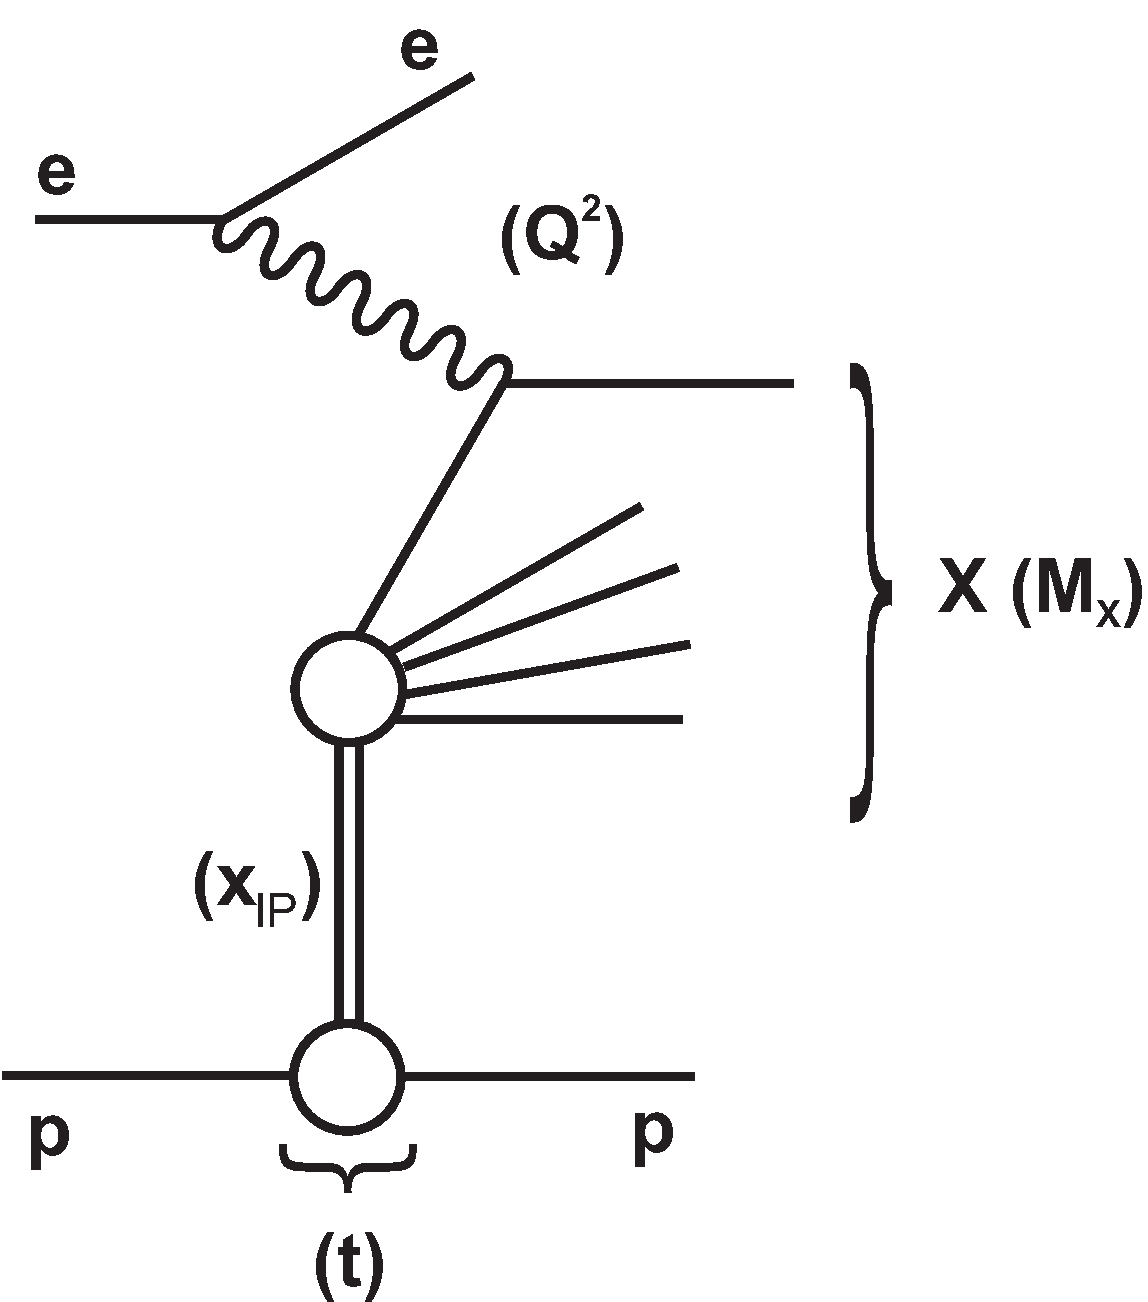
\includegraphics[width=0.5\linewidth]{figures/diffraction.pdf}
%\end{center}
%\caption{Schematic diagram of the kinematic variables used to
% describe the inclusive diffractive DIS process.}
%\label{fig:diff}
%\end{figure}

In addition to the usual variables $x$, $Q^2$, one must consider the squared four-momentum transfer $t$
(the undetected momentum transfer to the proton system) and
the mass $M_X$ of the diffractively produced final state. 
In practice, the variable $M_X$ 
is often replaced by $\beta=\frac{Q^2}{M_X^2+Q^2-t}$.
%
In models based on a factorisable pomeron, $\beta$ may be viewed as the fraction of the
pomeron longitudinal momentum which is carried by the struck parton, $x=\beta x_{\Pom}$.
%The diffractive parton distribution functions (DPDFs) are interpreted as probabilities for 
%finding a parton with a small fraction of the proton momentum $x=\beta\Pom$

For the inclusive case, the diffractive cross-section can be expressed as:
\begin{equation}
\begin{array}{lcl}
  \frac{d\sigma}{d\beta\,dQ^2dx_{\Pom}\,dt}
=
  \frac{2\pi\alpha^2}{\beta Q^4}\,
    \left( 1 +  (1-y)^2 \right) \ensuremath{\overline\sigma}^{D(4)}(\beta,Q^2,x_{\Pom},t)
\label{Dxs}
\end{array}
\end{equation}
where the ``reduced cross-section'' , $\overline\sigma$, is defined as
\begin{equation}
\begin{array}{lcl}
\overline\sigma^{D(4)}
 = F_2^{D(4)} - \frac{y^2}{1 +  (1-y)^2}\, F_L^{D(4)}.
% = F_T^{D(4)} + \frac{2(1-y)}{1 +  (1-y)^2}\, F_L^{D(4)}.
\label{eq:sigred}
\end{array}
\end{equation}
%The dimension of $F_k^{D(4)}(\beta,Q^2,x_{\Pom},t)$
%is $GeV^{-2}$ and thus quantities integrated over $t$.
%\begin{equation}
%F_k^{D(3)}(\beta,Q^2,x_{\Pom})
%\equiv
%\int_{t_{\rm min}}^{t_{\rm max}} dt
%F_k^{D(4)}(\beta,Q^2,x_{\Pom},t)
%\end{equation}
%are dimensionless. The maximum kinematically allowed value of $t$ is given by
%\begin{equation}
%t_{\rm MAX} 
%=
%-\frac{x_{\Pom}^2 m_p^2 + p_\perp^2}{1-x_{\Pom}}
%\approx 
%-\frac{x_{\Pom}^2}{1-x_{\Pom}} m_p^2
%\end{equation}
%where $m_p$ is the proton mass.
With $x = x_{\Pom}\beta$ we can relate this to the standard DIS formula.
%\begin{equation}
%\begin{array}{lcl}
%\frac{d\sigma}{d\beta\,dQ^2\,dx_{\Pom}\,dt} =
%  \frac{2\pi\alpha^2}{x\, Q^4}\,
%    \left( 1 +  (1-y)^2 \right) x_{\Pom}\ensuremath{\overline\sigma}^{D(4)}(\beta,Q^2,x_{\Pom},t)
%\end{array}
%\end{equation}
%which upon integration over $t$ reads
%\begin{equation}
%\begin{array}{lcl}
%\label{Dxs3}
%  \frac{d\sigma}{d\beta\,dQ^2\,dx_{\Pom}}
%=  
%  \frac{2\pi\alpha^2}{x Q^4}\,
%    \left( 1 +  (1-y)^2 \right) \,x_{\Pom}\ensuremath{\overline\sigma}^{D(3)}(\beta,Q^2,x_{\Pom}).
%\end{array}
%\end{equation}
%%The H1 and ZEUS data files typically contain $x_{\Pom}\ensuremath{\overline\sigma}^{D(3)}$.
The diffractive structure functions can be expressed as convolutions of the
calculable coefficient functions with diffractive quark and gluon distribution functions,
 which in general depend on \xpom, $Q^2$, $\beta$, $t$.

%==========================================
%{\bf Regge factorization} 
%Needed? \\
The diffractive PDFs in \fitter\ are implemented following the prescription of ZEUS
collaboration \cite{zeus:diff2009} and can be used to reproduce the main results.
%For a  better description of data, a contribution from a secondary Reggeon, $\Reg$, is included, hence
%\begin{equation}
%F_k^{D(4)}(\beta,Q^2,x_{\Pom},t) = 
%\sum_{\mathcal{X} =\Pom,\Reg}
%\phi_\mathcal{X}(x_{\Pom},t)\, F^\mathcal{X}_k(\beta,Q^2)
%\end{equation}
%or
%\begin{equation}
%\label{eq:FD3}
%F_k^{D(3)}(\beta,Q^2,x_{\Pom}) = 
%\sum_{\mathcal{X} =\Pom,\Reg}
%\Phi_\mathcal{X}(x_{\Pom})\, F^\mathcal{X}_k(\beta,Q^2)
%\end{equation}
%where
%\begin{equation}
%\label{eq:intFlux}
%\Phi_{\mathcal{X}}(x_{\Pom}) =
%\int\limits_{t_{\rm min}}^{t_{\rm max}} dt\, \phi_\mathcal{X}(x_{\Pom},t)
%\,.
%\end{equation}
%The fluxes are parametrized as
%\begin{subequations}
%\label{eq:flux}
%\begin{equation}
%\phi_\mathcal{X}(x_{\Pom},t) = 
%\frac {A_\mathcal{X}\, e^{b_\mathcal{X} t}} {x_{\Pom}^{2\alpha_\mathcal{X}(t) -1}}
%\end{equation}
%where
%\begin{equation}
%\alpha_\mathcal{X}(t) = \alpha_\mathcal{X}(0) + \alpha_\mathcal{X}' t
%\,.
%\end{equation}
%\end{subequations}
%The function $F^\Reg_k(\beta,Q^2)$  is taken to be that of the pion.
%




\subsection{Drell Yan processes  in $pp$ or $p\bar p$ collisions}
\label{dysection}

%This section presents calculations of Drell Yan processes that can be used to 
%predict lepton pair production at the LHC or Tevatron.
The Drell Yan (DY) process
provides further valuable information about PDFs.
In $pp$ and $p\bar p$ scattering, the $Z/\gamma\*$ and $W$ production 
probe bi-linear combinations of quarks. 
Complementary information on the different quark densities
can be obtained from the $W$ asymmetry ($d$, $u$ and their ratio),
the ratio of the $W$ and $Z$ cross sections (sensitive to the flavor 
composition of the quark sea, in particular to the $s$ density), 
and associated $W$ and $Z$ production with
heavy quarks (sensitive to $s$ and $c$ quark densities).
%

Presently, the predictions for Drell-Yan and $W$ and $Z$ production are available
to NNLO and $W$, $Z$ in association with heavy flavour quarks - to NLO. There are several possibilities 
for obtaining the theoretical
predictions for DY production in \fitter. 
At LO an analytic calculation is available within the package and described
below: 

The LO DY triple differential cross section in
invariant mass \(M\), boson rapidity \(y\) and Centre-of-Mass 
lepton Scattering (CMS) angle \(\cos\theta\), for NC, 
can be written as~\cite{Drell:1970wh,Yamada:1981mw}:
\begin{align}
% \scriptstyle
 \textstyle
% \frac{\mathrm{d}^3\sigma}{\mathrm{d}M\mathrm{d}y\mathrm{d}\cos\theta} &= 
 \frac{d^3\sigma}{dM{d}y d\cos\theta} =  
 \frac{\pi\alpha^2}{3MS}\sum_{q}P_q \left[f_q(x_1,Q^2)f_{\bar{q}}(x_2,Q^2) 
 + (q\leftrightarrow\bar{q})\right],
\end{align}
where \(S\) is the squared CMS beam energy, \(x_{1,2} = \frac{M}{\sqrt{S}}\exp(\pm y)\), $f_q(x_1,Q^2)$ 
is the parton number density, and 
$P_q$ is a partonic cross section. 
%\begin{align}
%  P_q &=  e_l^2e_q^2(1+\cos^2\theta) \nonumber \\
%      &+  e_le_q\frac{2M^2(M^2-M_Z^2)}{\sin^2\theta_W\cos^2\theta_W
%          \big[(M^2-M_Z^2)^2+\Gamma_Z^2M_Z^2\big]} \nonumber \\
%      &    \big[aA_q(1+\cos^2\theta)+2bB_q\cos\theta\big] \nonumber \\
%      &+  \frac{M^4}{\sin^4\theta_W\cos^4\theta_W
%          \big[(M^2-M_Z^2)^2+\Gamma_Z^2M_Z^2\big]} \nonumber \\
%      &    \big[(a^2+b^2)(A_q^2+B_q^2)(1+\cos^2\theta)+8abA_qB_q\cos\theta\big].
%\end{align}
%Here \(\theta_W\) is the Weinberg angle, \(M_Z\) and \(\Gamma_Z\) are Z boson mass and 
%width, $a, b, A_q, B_q, e_l, e_q$ are electro-weak couplings.
%
%\begin{align}
% a & = -\frac{1}{4} + \sin^2\theta_W, \  b  = -\frac{1}{4}, \nonumber \\
% A_q & = \frac{1}{2}I_q^3-e_q\sin^2\theta_W, \ B_q  = \frac{1}{2}I_q^3, \ I_u^3  = -I_d^3 = \frac{1}{2},  \nonumber \\
% e_l & = -1, e_u = \frac{2}{3}, e_d = -\frac{1}{3}.
%\end{align}
\\
\\
The expression for CC  scattering has a form:
\begin{align}
\frac{d^3\sigma}{dMdyd\cos\theta} &=
 \frac{\pi\alpha^2}{48S\sin^4\theta_W}
 \frac{M^3(1-\cos\theta)^2}{(M^2-M_W^2)+\Gamma_W^2M_W^2}  \nonumber \\
 & \sum_{q_1,q_2}V_{q_1q_2}^2f_{q_1}(x_1,Q^2)f_{q_2}(x_2,Q^2),
\end{align}
where \(V_{q_1q_2}\) is the CKM quark mixing matrix and \(M_W\) and \(\Gamma_W\)
are the \(W\) boson mass and decay width.

The simple form of these expressions allows the calculation of integrated
cross sections without the use of Monte-Carlo (MC) techniques which often 
introduce statistical fluctuations.
%This is particularly useful for PDF fitting purposes because
%statistical fluctuations are avoided in this case. 
In both NC and CC expressions PDFs
factorise as functions dependent only on boson rapidity \(y\) and
invariant mass \(M\), while
the integral in \(\cos\theta\) can be computed analytically.
%and integrations in \(y\) and \(M\) can be performed with the Simpson
%method. The \(\cos\theta\) parts are kept in the equation 
%explicitly because their integration is asymmetric for
%data in lepton \(\eta\) bins and also because of the need to apply 
%lepton \(p_{\perp}\) cuts.
%{\bf I think that this is an inappropriate level of detail about the LO DY calculation which could largely be replaced by references, however I have kept it for now, having moved it from the k-factor section where it did not belong}

The NLO and NNLO calculations are 
highly demanding
in terms of the computing power and time, and $k$-factor or fast grid techniques must be employed (see section~\ref{sec:techniques}
for details), interfaced to programs such as
\texttt{MCFM}~\cite{Campbell:1999ah,Campbell:2000je,Campbell:2010ff}, 
available for NLO calculations, or 
FEWZ~\cite{FEWZ} and DYNNLO \cite{DYNNLO} for NLO and NNLO.
 

%The most abundant processes at the LHC are the production of the $W$ and $Z$ bosons, therefore measurements of the $W$ and $Z$ cross-sections are very precise. Their  LO decomposition in terms of quark distributions show strong 


%Alternatively, one can obtain the NLO predictions directly by using 
%APPLGRID or FASTNLO techniques, which rely on the factorisation theorem by 
%decoupling the hard scattering coefficients from PDFs.
%The hard scattering coefficients are calculated once and stored into a grid 
%for a given kinematic bin, speeding up the convolution process with the PDFs 
%and thus allowing to for fast QCD fits. 


%These methods are described in more detail in section \ref{sec:theory:jets}.
%An independent treatment for the electro-weak corrections is applied as the 
%independent k-factors, using packages such as SANC and FEWZ.

\subsection{Jet production in $ep$ and $pp$ or $p \bar p$ collisions}
\label{jetsection}
%In this subsection, the use of the factorisation formalism is fully exploited for the 
%calculations of the inclusive jets and dijet cross sections.
%This sections presents various fast calculational techniques for jet production based on
%the factorization formalism.

Jet production at high transverse momentum is sensitive to the high-$x$ gluon 
PDF (see e.g.~\cite{MSTWpdf}) and can thus increase the precision of the 
gluon PDF determination, which is particularly important for the Higgs production and searches for new physics.
Jet production cross sections are currently only known to NLO, although NNLO 
calculations are now quite advanced~\cite{nigel:2013,nigel:2010,Currie:2013dwa}. 
Within \fitter programs \texttt{MCFM} and 
\nlojetpp~\cite{Nagy:1998bb,Nagy:2001fj} may be used for the 
calculation of jet production.
Similarly to the DY case, the calculation 
is very demanding in terms of computing power. 
Therefore fast grid techniques are used to efficiently perform PDF and
$\alpha_S$ fits of jet cross section measurements in $ep$, $pp$ and
$p\bar{p}$ collisions
%Therefore, to allow the possibility to include  $ep$, $pp$ or $p\bar p$ 
%jet cross section 
%measurements in QCD fits in order to extract PDFs and $\as$, the fast 
%grid techniques are used 
(for details see section~\ref{sec:techniques}).


%the perturbative
%coefficients have to be pre-computed in a PDF and $\alpha_s$ 
%independent way. For this reason, the fast grid tools to the theory calculations
%obtained with MCFM~\cite{Campbell:1999ah,Campbell:2000je,Campbell:2010ff} and NLOJET++~\cite{Nagy:1998bb,Nagy:2001fj}, 
%which are interfaced to the \fitter , are also exploited for the jet production . 



\subsection{Top-quark production in $pp$ and $p \bar p$ collisions}

Top-quark pairs ($t \bar t$) are produced at hadron colliders dominantly via $gg$ fusion 
and $q \bar q$ annihilation. Measured $t \bar t$ cross sections provide additional 
constraints in particular on the gluon density at medium to high values of $x$, 
on $\as$ and on the top-quark mass, $m_t$. 
Single top quarks are produced via electroweak interactions and single-top cross sections 
can be used, for example, to probe the ratio of the $u$ and $d$ densities in the proton 
as well as the $b$-quark PDF.
Precise predictions for the total $t \bar t$ cross section have become available 
to full NNLO recently~\cite{Czakon:2013goa}. They can be used within \fitter via an interface 
to the program \texttt{HATHOR}~\cite{Aliev:2010zk}. Differential $t \bar t$ cross sections and predictions 
for single-top production can be used with \fitter at NLO accuracy from 
\texttt{MCFM}~\cite{Campbell:2010ff,Campbell:2009ss,Campbell:2005bb,Campbell:2004ch,Campbell:2012uf} 
in combination with fast grid techniques.

%\subsection{Cross Sections for \texorpdfstring{$t\bar{t}$}{t-tbar} production in $pp$ or $p\bar p$ collisions}
%
%This provides the possibility to use top production to
%constrain the gluon density in the proton. Calculations are available to NLO precision with  
%MCFM and to approximate NNLO precision with the HATHOR program~\cite{Aliev:2010zk}. These are both available within \fitter\. 
%Version 1.3 of HATHOR includes the exact NNLO for $q \bar q \to t \bar t$ \cite{Baernreuther:2012ws}
%as well as a new high-energy constraint on the 
%approximate NNLO calculation obtained from
%soft-gluon resummation \cite{Moch:2012mk}.
%The use of these programs also requires fast grid techniques.
